\documentclass[12pt, a4papre]{article}
\usepackage[catalan]{babel}
\usepackage[unicode]{hyperref}
\usepackage{amsmath}
\usepackage{amssymb}
\usepackage{amsthm}
\usepackage{xifthen}
\usepackage{siunitx}
\usepackage{xcolor}
\usepackage{float}
\usepackage{listings}
\usepackage{setspace}
\usepackage{graphicx}
\usepackage{tikz,lipsum,lmodern}
\usepackage[most]{tcolorbox}
\usepackage{circuitikz}
\usepackage{indentfirst}
\usepackage{verbatimbox}
\definecolor{mygreen}{RGB}{28,172,0} % color values Red, Green, Blue
\definecolor{mylilas}{RGB}{170,55,241}

\graphicspath{ {./Fotos/} }


\newcommand{\norm}[1]{\lvert #1 \rvert}

\hypersetup{
    colorlinks = true,
    linkcolor = blue
}

\author{Daniel Vilardell}
\title{Previ 2 SSIS }
\date{}

\begin{document}
	\maketitle
	\section{}
	
	\textbf{a) i b)}
	
	Sabem que la transformada de fourier de $x(t) =  A\cos{(2\pi f_0 t)} $ es
	\[\mathcal{F}(x(t)) = \frac{1}{2}(\delta(f - f_0) + \delta(f - f_0))\]
	
	També sabem que si la multipliquem per la finestra $h(t)$ la transformada de Fourier del producte serà la convolució de les transformades de fourier individuals. Per tant considerem la transformada de fourier del pols rectangular i del pols triangular.
	
	\[\mathcal{F}(\prod(\frac{t}{T})) = Tsinc(Tf)\]
	\[\mathcal{F}(\Lambda(\frac{t}{\frac{T}{2}})) = \frac{T}{2} sinc^2(\frac{Tf}{2}) \]
	
	Com que la convolucio per una delta el que fa es desplaçar $f_0$ el resultat serà 
	
	\[\mathcal{F}(x(t))*\mathcal{F}(\prod(\frac{t}{T})) = \frac{AT}{2}(sinc(T(f - f_0)) + sinc(T(f + f_0)))\]
	
	\[\mathcal{F}(x(t))*\mathcal{F}(\Lambda(\frac{t}{\frac{T}{2}})) = \frac{AT}{4}(sinc^2(\frac{T}{2}(f - f_0)) + sinc^2(\frac{T}{2}(f + f_0)))\]
	
	\newpage
	\textbf{c)}
	\begin{figure}[H]
		\begin{center}
		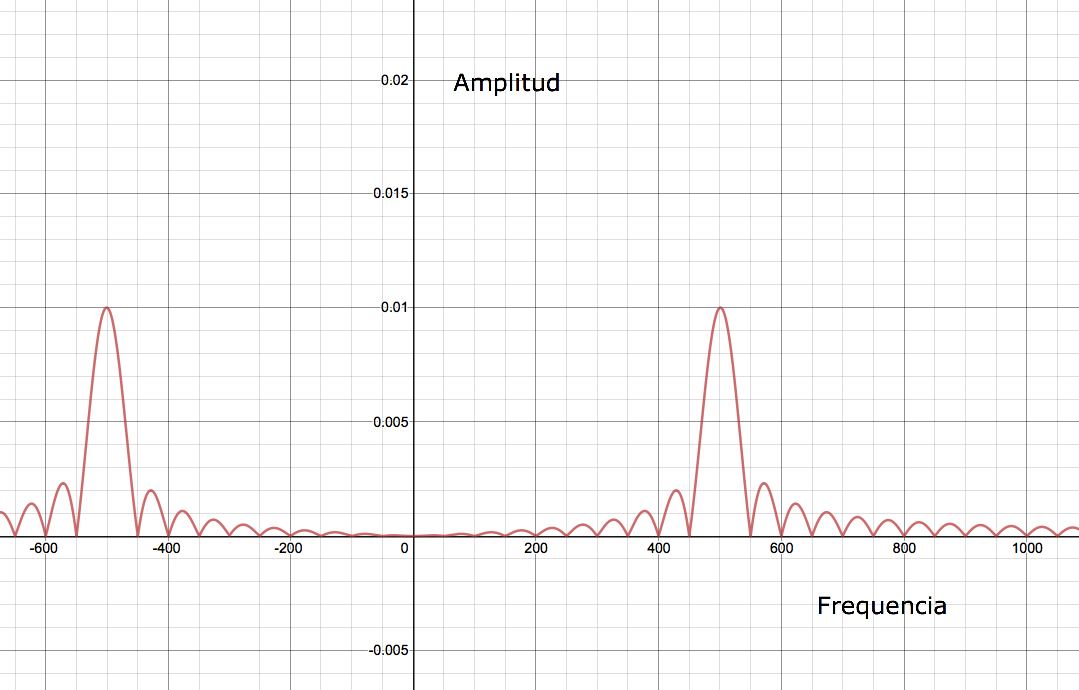
\includegraphics[width=130mm]{graficaSSIS1.png}
		\end{center}
		\caption{$\mathcal{F}(x(t))*\mathcal{F}(\prod(\frac{t}{T}))$}
	\end{figure}
	
	Sabem que $sinc(x)$ te valor maxim 1, per tant si multipliquem el resultat per 0.01, el valor maxim que prendra serà 0.01. Això tindrà lloc a les frequencies $-500Hz$ i $500Hz$. 
	
	Com també hem vist a teoria, l'amplada del lobul principal en un pols rectangular de frequencia $T$ es de $\frac{2}{T}$ on d es la durada de la finestra. Per tant la amplada en el nostre cas serà de $\frac{2}{0.02} = 100Hz$. Per tant les frequencies exactes dels 0 mes propers als maxims seran $-450Hz$, $-550Hz$, $550Hz$ i $450Hz$.
	
	També vist a teoria la relació entre el maxim del lobul principal i el secundari serà de 13dB, i per tant el quocient serà $10^{-\frac{13}{20}} = 0.22$.
	
	\begin{figure}[H]
		\begin{center}
		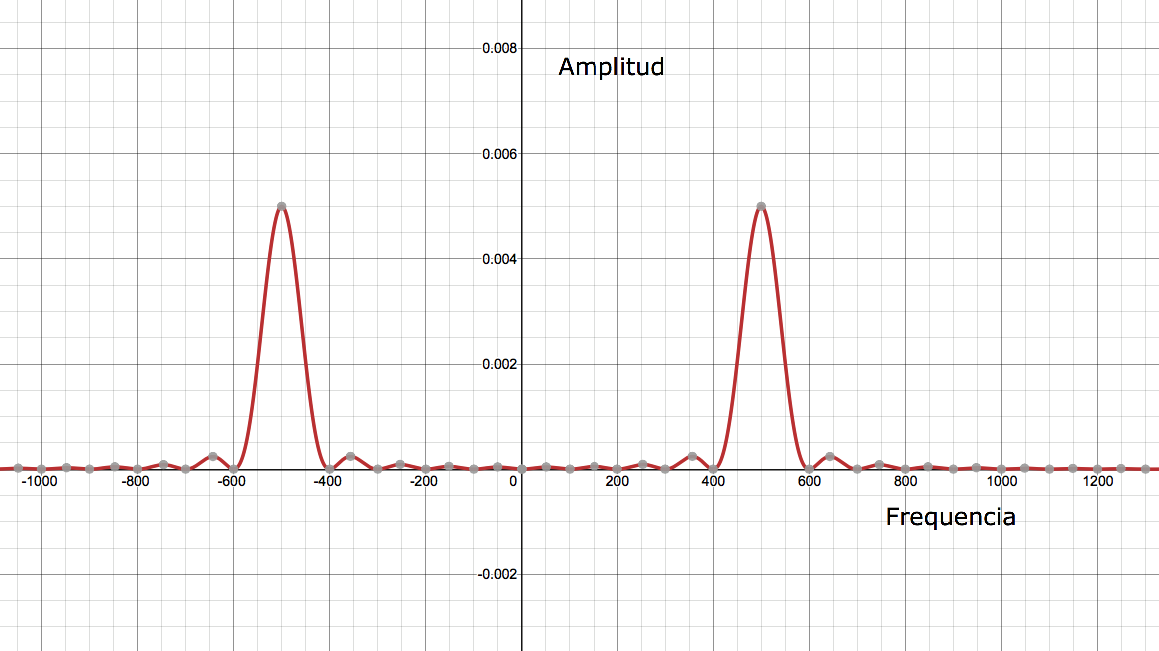
\includegraphics[width=130mm]{graficaSSIS3.png}
		\end{center}
		\caption{$\mathcal{F}(x(t))*\mathcal{F}(\Lambda(\frac{t}{\frac{T}{2}}))$}
	\end{figure}
	
	Sabem que $sinc(x)$ te valor maxim 1, per tant si multipliquem el resultat per 0.005, el valor maxim que prendra serà 0.005. Això tindrà lloc a les frequencies $-500Hz$ i $500Hz$.
	
	 Com també hem vist a teoria, l'amplada del lobul principal en un pols rectangular de frequencia $T$ es de $\frac{4}{T}$ on d es la durada de la finestra. Per tant la amplada en el nostre cas serà de $\frac{4}{0.02} = 200Hz$. Per tant les frequencies exactes dels 0 mes propers als maxims seran $-400Hz$, $-600Hz$, $600Hz$ i $400Hz$.
	
	També vist a teoria la relació entre el maxim del lobul principal i el secundari serà de 13dB, i per tant el quocient serà $10^{-\frac{26}{20}} = 0.05$.
	
	\newpage
	\section{}
	
	\textbf{a) i b)}
	
	Ara fem el mateix per a $x(t) = A\cos(2\pi f_0t) + B\cos(2\pi f_1t)$. Calculem en primer lloc la seva transformada, aplicant la propietat de linealitat de les transformades de Fourier.
	
	\[\mathcal{F}(x(t)) = \frac{1}{2}(\delta(f - f_0) + \delta(f - f_0) + \delta(f - f_1) + \delta(f - f_1)) \]
	
	Ara amb les mateixes finestres que el apartat anterior calculem la convolucio de les seves transformades
	
	
	\[
	\begin{aligned}
	\mathcal{F}(x(t))*\mathcal{F}(\prod(\frac{t}{T})) =   \frac{T}{2}(Asinc(T(f - f_0)) + Asinc(T(f + f_0)& + Bsinc(T(f - f_1)) + \\
      &+ Bsinc(T(f + f_1)))
	\end{aligned}
	\]	
	\[
	\begin{aligned}
	\mathcal{F}(x(t))*\mathcal{F}(\Lambda(\frac{t}{\frac{T}{2}})) =   \frac{T}{4}(Asinc^2(&\frac{T}{2}(f - f_0)) + Asinc^2(\frac{T}{2}(f + f_0)) +  \\
      &  + Bsinc^2(\frac{T}{2}(f - f_1)) + Bsinc^2(\frac{T}{2}(f + f_1)))
	\end{aligned}
	\]
	
	\newpage
	\textbf{c)}
	\begin{figure}[H]
		\begin{center}
		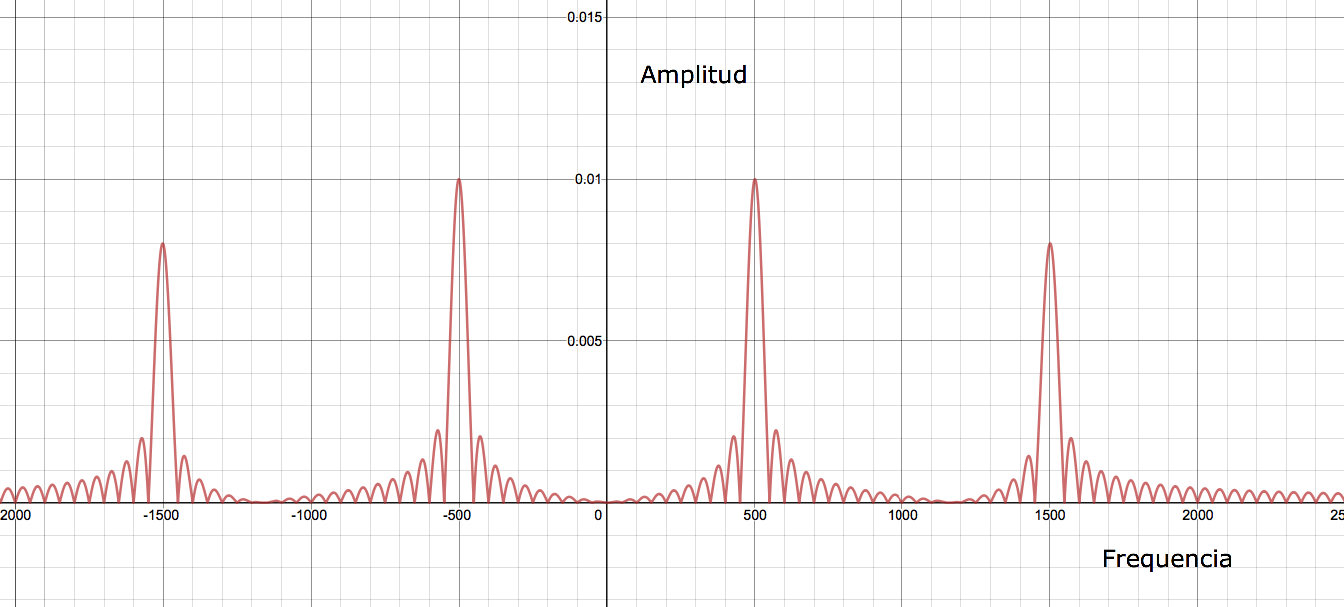
\includegraphics[width=120mm]{graficaSSIS2.png}
		\end{center}
		\caption{$\mathcal{F}(x(t))*\mathcal{F}(\prod(\frac{t}{T}))$}
	\end{figure}
	
	Per les mateixes raons que abans, la funcio te dos maxims a $500Hz$ i $-500Hz$ de amplitud 0.1 i dos maxims a $1500Hz$ i $-1500Hz$ de amplitud 0.08. Al mantenir $T = 20ms$ es mantindrà l'amplada de banda dels diferents lobuls, es a dir $100Hz$. Finalment la relacio entre el lobul principal i el secundari serà la mateixa, es a dir 0.22.
	
	\begin{figure}[H]
		\begin{center}
		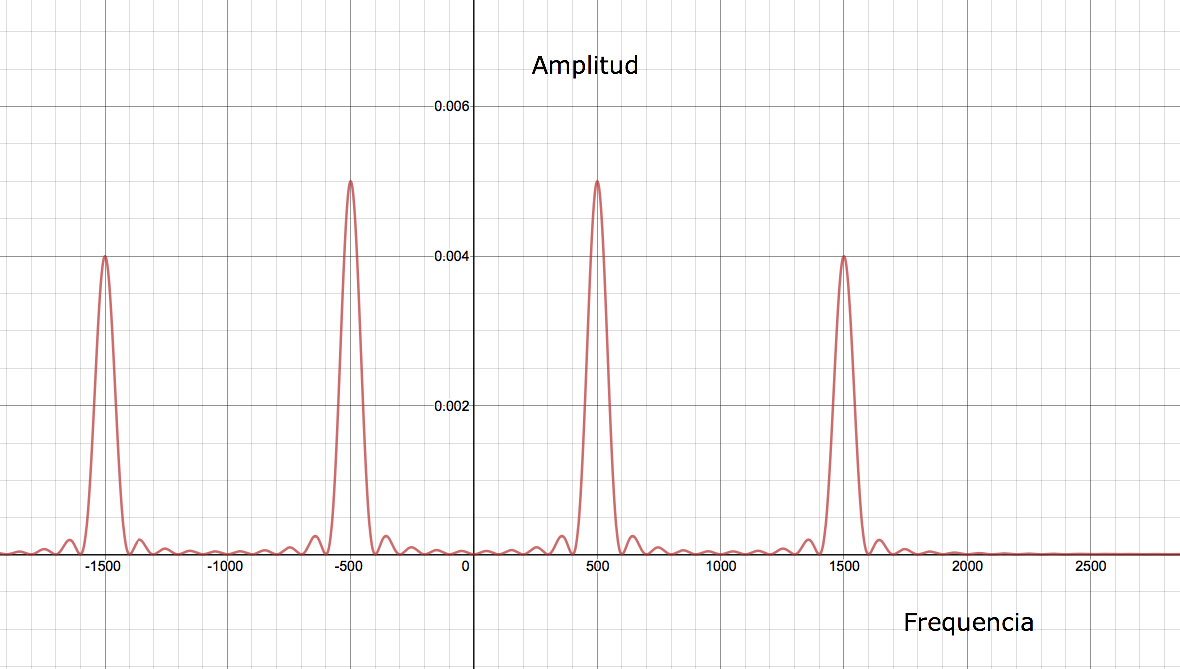
\includegraphics[width=120mm]{graficaSSIS4.png}
		\end{center}
		\caption{$\mathcal{F}(x(t))*\mathcal{F}(\Lambda(\frac{t}{\frac{T}{2}}))$}
	\end{figure}
	
	Per les mateixes raons que abans, la funcio te dos maxims a $500Hz$ i $-500Hz$ de amplitud 0.05 i dos maxims a $1500Hz$ i $-1500Hz$ de amplitud 0.04. Al mantenir $T = 20ms$ es mantindrà l'amplada de banda dels diferents lobuls, es a dir $200Hz$. Finalment la relacio entre el lobul principal i el secundari serà la mateixa, es a dir 0.05.
	
	\newpage
	\section{}
	\textbf{a)}
	
	La senyal de entrada  serà $x(t)=\cos{t}$ i la senyal de sortida  $y(t)=a\cos{t} + b\cos^2{t}$.  Ja vam veure a MATEL que la transformada de $x(t)=\cos{t}$ es 
	\[\mathcal{F}(x(t)) = \frac{1}{2}(\delta(f - \frac{1}{2\pi}) + \delta(f + \frac{1}{2\pi}))\]
	
	La transformada del senyal de sortida serà
	\[\mathcal{F}(y(t)) = \frac{a}{2}(\delta(f - \frac{1}{2\pi}) + \delta(f + \frac{1}{2\pi})) + b\mathcal{F}(x(t))*\mathcal{F}(x(t)) \]
	
	Per tant nomes ens caldrà calcular la convolucio de deltes.
	\[b\mathcal{F}(x(t))*\mathcal{F}(x(t)) = \frac{b}{4}(\delta(f - \frac{1}{\pi}) + \delta(f + \frac{1}{\pi})) + 2\delta(f) \]
	
	Així doncs es pot veure que el sistema el que fa a la transformada es variar les amplituds de les deltes de la transformada original, i n'afegeix dos mes de amplitud $\frac{b}{4}$ a frequencies $-\frac{1}{\pi}$ i $\frac{1}{\pi}$, i una al 0 amb amplitud $\frac{b}{2}$.
	
	\textbf{b)}
	
	Per a fer aquest apartat primer farem el \textbf{2.} i despres amb la informacio del 2 farem el  \textbf{1.}
	
	 \textbf{2.} Considerem $x(t)=\cos{2\pi f_0t}$ i una senyal $h(t)$ lineal e invariant. Per a calcular la senyal resultant de aplicar $x(t)$ al sistema usarem la propietat de les transformades de fourier que diu que la transformada del producte de funcions es la convolucio de transformades de les funcions per separat. 
	 \[\mathcal{F}(y(t)) = X(f)H(f) = X(f)|H(f)|e^{j\phi(H(f))} = \frac{1}{2} |H(f)|(\delta(f - f_0) + \delta(f + f_0))e^{j\phi(H(f))}\]
	 
	 I per tant la antitransformada es inmediata
	 \[y(t)=|H(f_0)|cos(2\pi f_0t + \phi(H(f)))\]

	\textbf{1.} Calculem ara doncs la transformada de $h(t) = -2\delta(t) + 5e^{-2t}u(t)$
	\[\mathcal{F}(h(t)) = -2 + \frac{5}{2 + j2\pi f}\]
	
	Que te com a fase a $f_0 = \frac{1}{2\pi}$ $\phi(H(f)) = \pi - (0 - argtg(\frac{2\pi f_0}{2})) = 2.67rad$ i modul 3. Per tant la sortida del sistema es
	\[y(t) = 3cos(t + 2.67)\]
	
	 \textbf{3.} No es pot aplicar a un sistema no lineal ja que no podriem descompondre la transformada de $h(t)$ en modul i fase de la manera que ho hem fet a  \textbf{2}.
	
	
\end{document}




